\section{Antecedentes}
\label{ch:2:section:background}

% region historia
\subsection{Historia, línea temporal}

%https://www.techtarget.com/searchenterpriseai/tip/The-history-of-artificial-intelligence-Complete-AI-timeline

A continuación, se describe la línea de temporal con los hitos más relevantes en el desarrollo de la inteligencia artificial, sus avances hasta él \gls{DL} y como se ha llegado a las redes neuronales actuales o la inteligencia artificial generativa. Se han adjuntado referencias de las investigaciones, artículos y publicaciones realizadas. \cite{TIMELINE-schmidhuber2022annotated}

Como podemos observar en la línea temporal de la figura \ref{tab:timeline} se realizaron grandes avances en este campo desde principios del siglo \miscrom{XVII}, partiendo de las bases matemáticas como la regla de la cadena, pasando por la teoría Hebbiana hasta nuestros días con los modelos de redes neuronales. Haremos un recorrido de los avances más relevante y su contribución.

Describiremos de forma breve el funcionamiento técnico de los avances más significativos en redes neuronales y visión por computador, para posteriormente explicar las distintas formas de diseñar una red neuronal adversarial generativa.

\begin{table}
    \centering
    \rule{\linewidth}{1pt}
        \ytl{1676     }{The Chain Rule \cite{leibniz2012early}                                                    }
        \ytl{1847     }{Augustin-Louis Cauchy \cite{lemarechal2012cauchy}                                         }
        \ytl{1943     }{Threshold Logic Unit (TLU) \cite{mcculloch1943logical}                                    }
        \ytl{1949     }{Teoría Hebbiana                                                                           }
        \ytl{1958     }{Perceptron \cite{rosenblatt1958perceptron}                                                }
        \ytl{1959-1960}{Adaline y Madaline \cite{rosenblatt1958perceptron}                                        }
        \ytl{1965     }{Multilayer Perceptron (MLP) \cite{baum1988capabilities}                                   }
        \ytl{1967-1968}{Deep Learning by Stochastic Gradient Descent \cite{karplus19671967}                       }
        \ytl{1980`s   }{
            Neuronas Sigmoidales                                            \\
            Feedforward neural network (FNN) \cite{rumelhart1985learning}   \\
            Backpropagation (BP) \cite{rosenblatt1962principles,etde_5080493,lecun1985learning}
        }
        \ytl{1985     }{Boltzmann Machine \cite{ACKLEY1985147}                                                    }
        \ytl{1987     }{Adaptive resonance theory (ART) \cite{grossberg1987competitive}                           }
        \ytl{1989     }{
                        Convolutional neural networks (CNN) \cite{lecun1989backpropagation} \\
                        Recurent neural networks (RNN) \cite{schmidhuber1993habilitation}     
        }
        \ytl{1990     }{Generative Adversarial Networks (GAN) as Game \cite{schmidhuberunsupervised}              }
        \ytl{1997     }{Long short term memory (LSTM) \cite{Hochreiter1997LongSM, hochreiter1997long}             }
        \ytl{2006     }{
            Deep Belief Networks (DBN) \cite{hinton2006fast}            \\
            Restricted Boltzmann Machine \cite{hinton2006reducing}      \\
            Encoder / Decoder (Auto-encoder) \cite{hinton2006reducing}                                
        }
        \ytl{2014     }{Generative Adversarial Networks (GAN) Moderns \cite{6294131,goodfellow2014generative}     }
        \ytl{2018     }{Style Generative Adversarial Networks (Style-GAN) \cite{karras2019stylebased}             }
    \bigskip
    \rule{\linewidth}{1pt}%
    \caption{Hitos de las redes neuronales artificiales}
    \label{tab:timeline}
\end{table}



\newpage
\subsection{Historia de la Inteligencia Artificial}

Todo surge en 1676 por {Gottfried Wilhelm Leibniz} \ref{fig:gottfried-leibniz} publicó la regla de la cadena del cálculo diferencial, esencial para el análisis matemático, es la esencial para calcular como cambiará la función final si se cambian los pesos de funciones anteriores.

La regla de la cadena es fundamental para técnicas como el descenso de gradiente, propuesto por {Augustin-Louis Cauchy} en 1847 y utilizado para ajustar iterativamente los pesos de una \acrshort{NN} durante el entrenamiento.
Posteriormente en 1805 {Adrien-Marie Legendre} y {Johann Carl Friedrich Gauss} desarrollaron \acrshort{NN}, matemáticamente eran regresiones lineales muy simples, similares a las redes neuronales lineales simples.
Esto lo uso {Gauss} para redescubrir el planeta enano Ceres.

\begin{figure}[H]
    \centering
    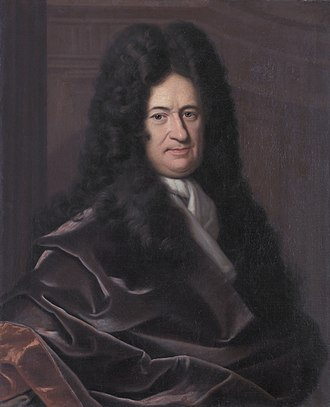
\includegraphics[width=0.45\textwidth]{figures/Gottfried_Wilhelm_Leibniz,_Bernhard_Christoph_Francke.jpg}
    \caption{Retrato de Gottfried Leibniz.\newline{}Fuente: \href{https://es.wikipedia.org/wiki/Gottfried_Leibniz}{Wikipedia}}
    \label{fig:gottfried-leibniz}
\end{figure}

Aunque realmente la historia comienza en 1943 con la investigación de {Warren McCulloch} y {Walter Pitss}, publicaron el artículo \textit{A logical calculus of the ideas immanent in nervous activity} \cite{mcculloch1943logical}.
Dicho artículo creó distintas ramas de investigación (ordenadores digitales, inteligencia artificial, funcionamiento del perceptron).

\begin{figure}[H]
    \centering
    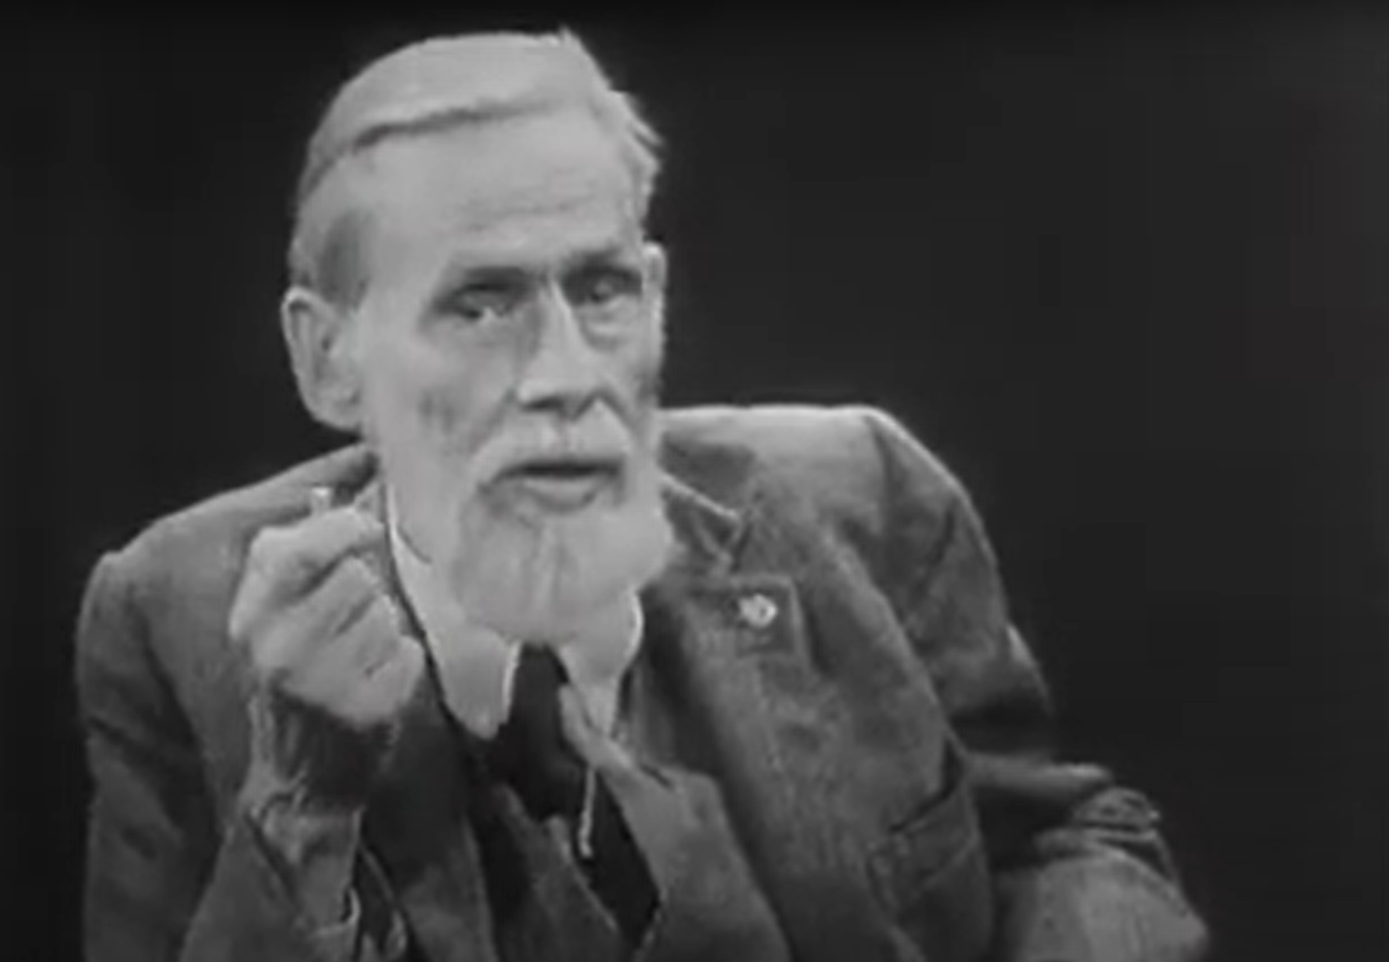
\includegraphics[width=0.55\textwidth]{figures/Warren Sturgis McCulloch Interview.png}
    \caption{Warren Sturgis McCulloch Interview.\newline{}Fuente: \href{https://www.youtube.com/watch?v=8Wdz1Tj5084}{Entrevista en 1969}}
    \label{fig:Warren Sturgis McCulloch}
\end{figure}


En 1956 en la primera conferencia de inteligencia artificial organizada por la fundación {Rochester}, se reúnen los investigadores fundadores de los conceptos actuales de la IA ({Minsky, McCarthy, Rochester, Shanon}), gran parte de la bibliografía se refiere a este punto como el origen y contacto de las redes neuronales artificiales.
En dicha conferencia (\textit{Nathaural Rochester}) presento el modelo de una red neuronal que fue el resultado de la investigación desarrollada por el equipo de investigación de IBM.

\begin{figure}[H]
    \centering
    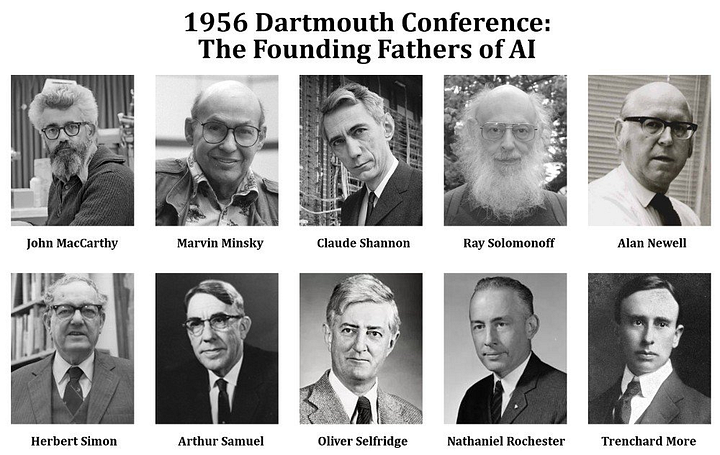
\includegraphics[width=0.75\textwidth]{figures/conferecia 1956 - 1689170718524.png}
    \caption{Los padres de la inteligencia artificial.\newline{}Fuente: \href{https://www.linkedin.com/pulse/first-ever-ai-conference-tracing-evolution-history-ofai-nicky-verd}{Linkedin}}
    \label{fig:conferencia-1956}
\end{figure}

En 1957 se presenta el ``\textit{Perceptron}'' por {Frank Rosenblatt}, dicho elemento es un sistema clasificador de patrones, además contaba con la capacidad de aprender, de ser robusto matemáticamente y poder adaptarse si algún componente se dañaba.

\begin{figure}[H]
    \centering
    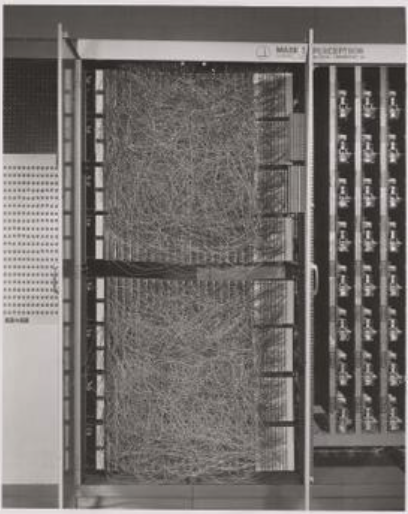
\includegraphics[width=0.4\textwidth]{figures/perceptron.png}
    \caption{Mark I Perceptron.\newline{}Fuente: \href{https://en.wikipedia.org/wiki/Perceptron}{Wikipedia}}
    \label{fig:perceptron}
\end{figure}

El \textit{Perceptron} fue diseñado originalmente para el reconocimiento óptico usando un sistema de 400 fotocélulas en rejilla.
Posteriormente, se describió el problema de no-linealidad que presentaban los perceptrones (Problema XOR) \cite{cuevastello2018apuntes}.

De 1959 a 1960 {Bernard Widrow} y {Ted Hoff} desarrollaron ``Adaline'' y ``Madaline'' \cite{widrow1960adaptive} que resolvía el problema de la no-linealidad y que tenía aplicación en el reconocimiento de voz, series temporales, caracteres, etc.

Posteriormente, el \textit{MIT} realizo una investigación matemática muy crítica de todos los problemas que presentaba el \textit{Perceptron} llegando a la conclusión que tenían grandes problemas que no podrían ser resueltos, por lo que en la próxima década (años 60) se redujo drásticamente las investigaciones sobre el campo de las redes neuronales.
Esto llevo a uno de los famosos inviernos de la inteligencia artificial (1974 - 1980).

\begin{figure}[H]
    \centering
    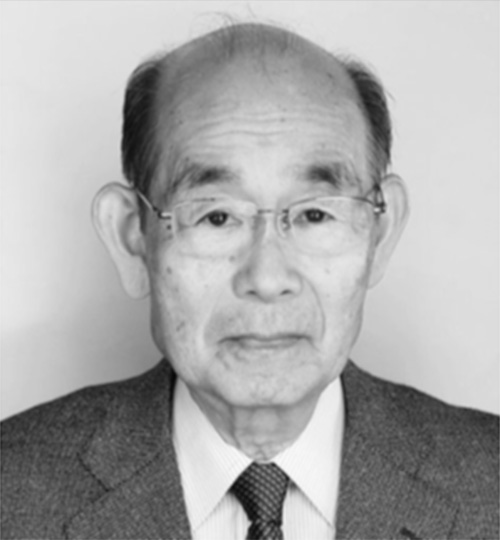
\includegraphics[width=0.25\textwidth]{figures/Kunihiko Fukushima.jpg}
    \caption{Kunihiko Fukushima.\newline{}Fuente: \href{https://www.ieice.org/eng/about_ieice/new_honorary_members_award_winners/2017/meiyo_05e.html}{IEICE}}
    \label{fig:kunihiko-fukushima}
\end{figure}

Durante la década de los 70 se hacen aportes a la teoría \textit{Hebbiana}, se aportan logros en al análisis y descripción de reglas adaptativas, además de otros aportes al principio de aprendizaje competitivo.
En 1979 presentó {Kunihiko Fukushima} la primera red neuronal \gls{CNN}, la llamó Neocognitron \cite{fukushima1979neural}, dicho trabajo en un futuro se mejoraría con técnicas de \gls{BP-NN}.

En la década de los 80 se realizaron aportes como el algoritmo de \gls{BP-NN} que surgió del artículo de {Hopfield} \cite{hopfield1982neural}, esto despertó la curiosidad de muchos investigadores a volver al campo de las redes neuronales.
Se realizaron aportes como las redes \gls{GNN}.
La investigación continuó con {Stephen Grossberg} que realizo aportes derivados de estudios fisiológicos de cómo funcionaban las neuronas y la plasticidad, lo que permitió la creación de reglas y postulados, esto se ve en los trabajos de las redes \acrshort{ART-NN} \cite{grossberg1987competitive}.
La investigación de {Hopfield} basada en el trabajo de {Stephen Grossberg} creo un sistema computacional neuronal interconectado que tiende a un mínimo de energía.
En 1985 {David E. Rumelhart} basándose en la investigación realizada por {Paul Werbos} \cite{etde_5080493} realizo un análisis experimental del algoritmo \gls{BP-NN} y su aplicación en redes \acrshort{FNN} \cite{rumelhart1985learning}.

{Yann LeCun} junto a su equipo, en 1989 crearon la primera aplicación \acrshort{CNN} con técnicas \acrshort{BP} dicha aplicación podía reconocer números a partir de imágenes.

\begin{figure}[H]
    \centering
    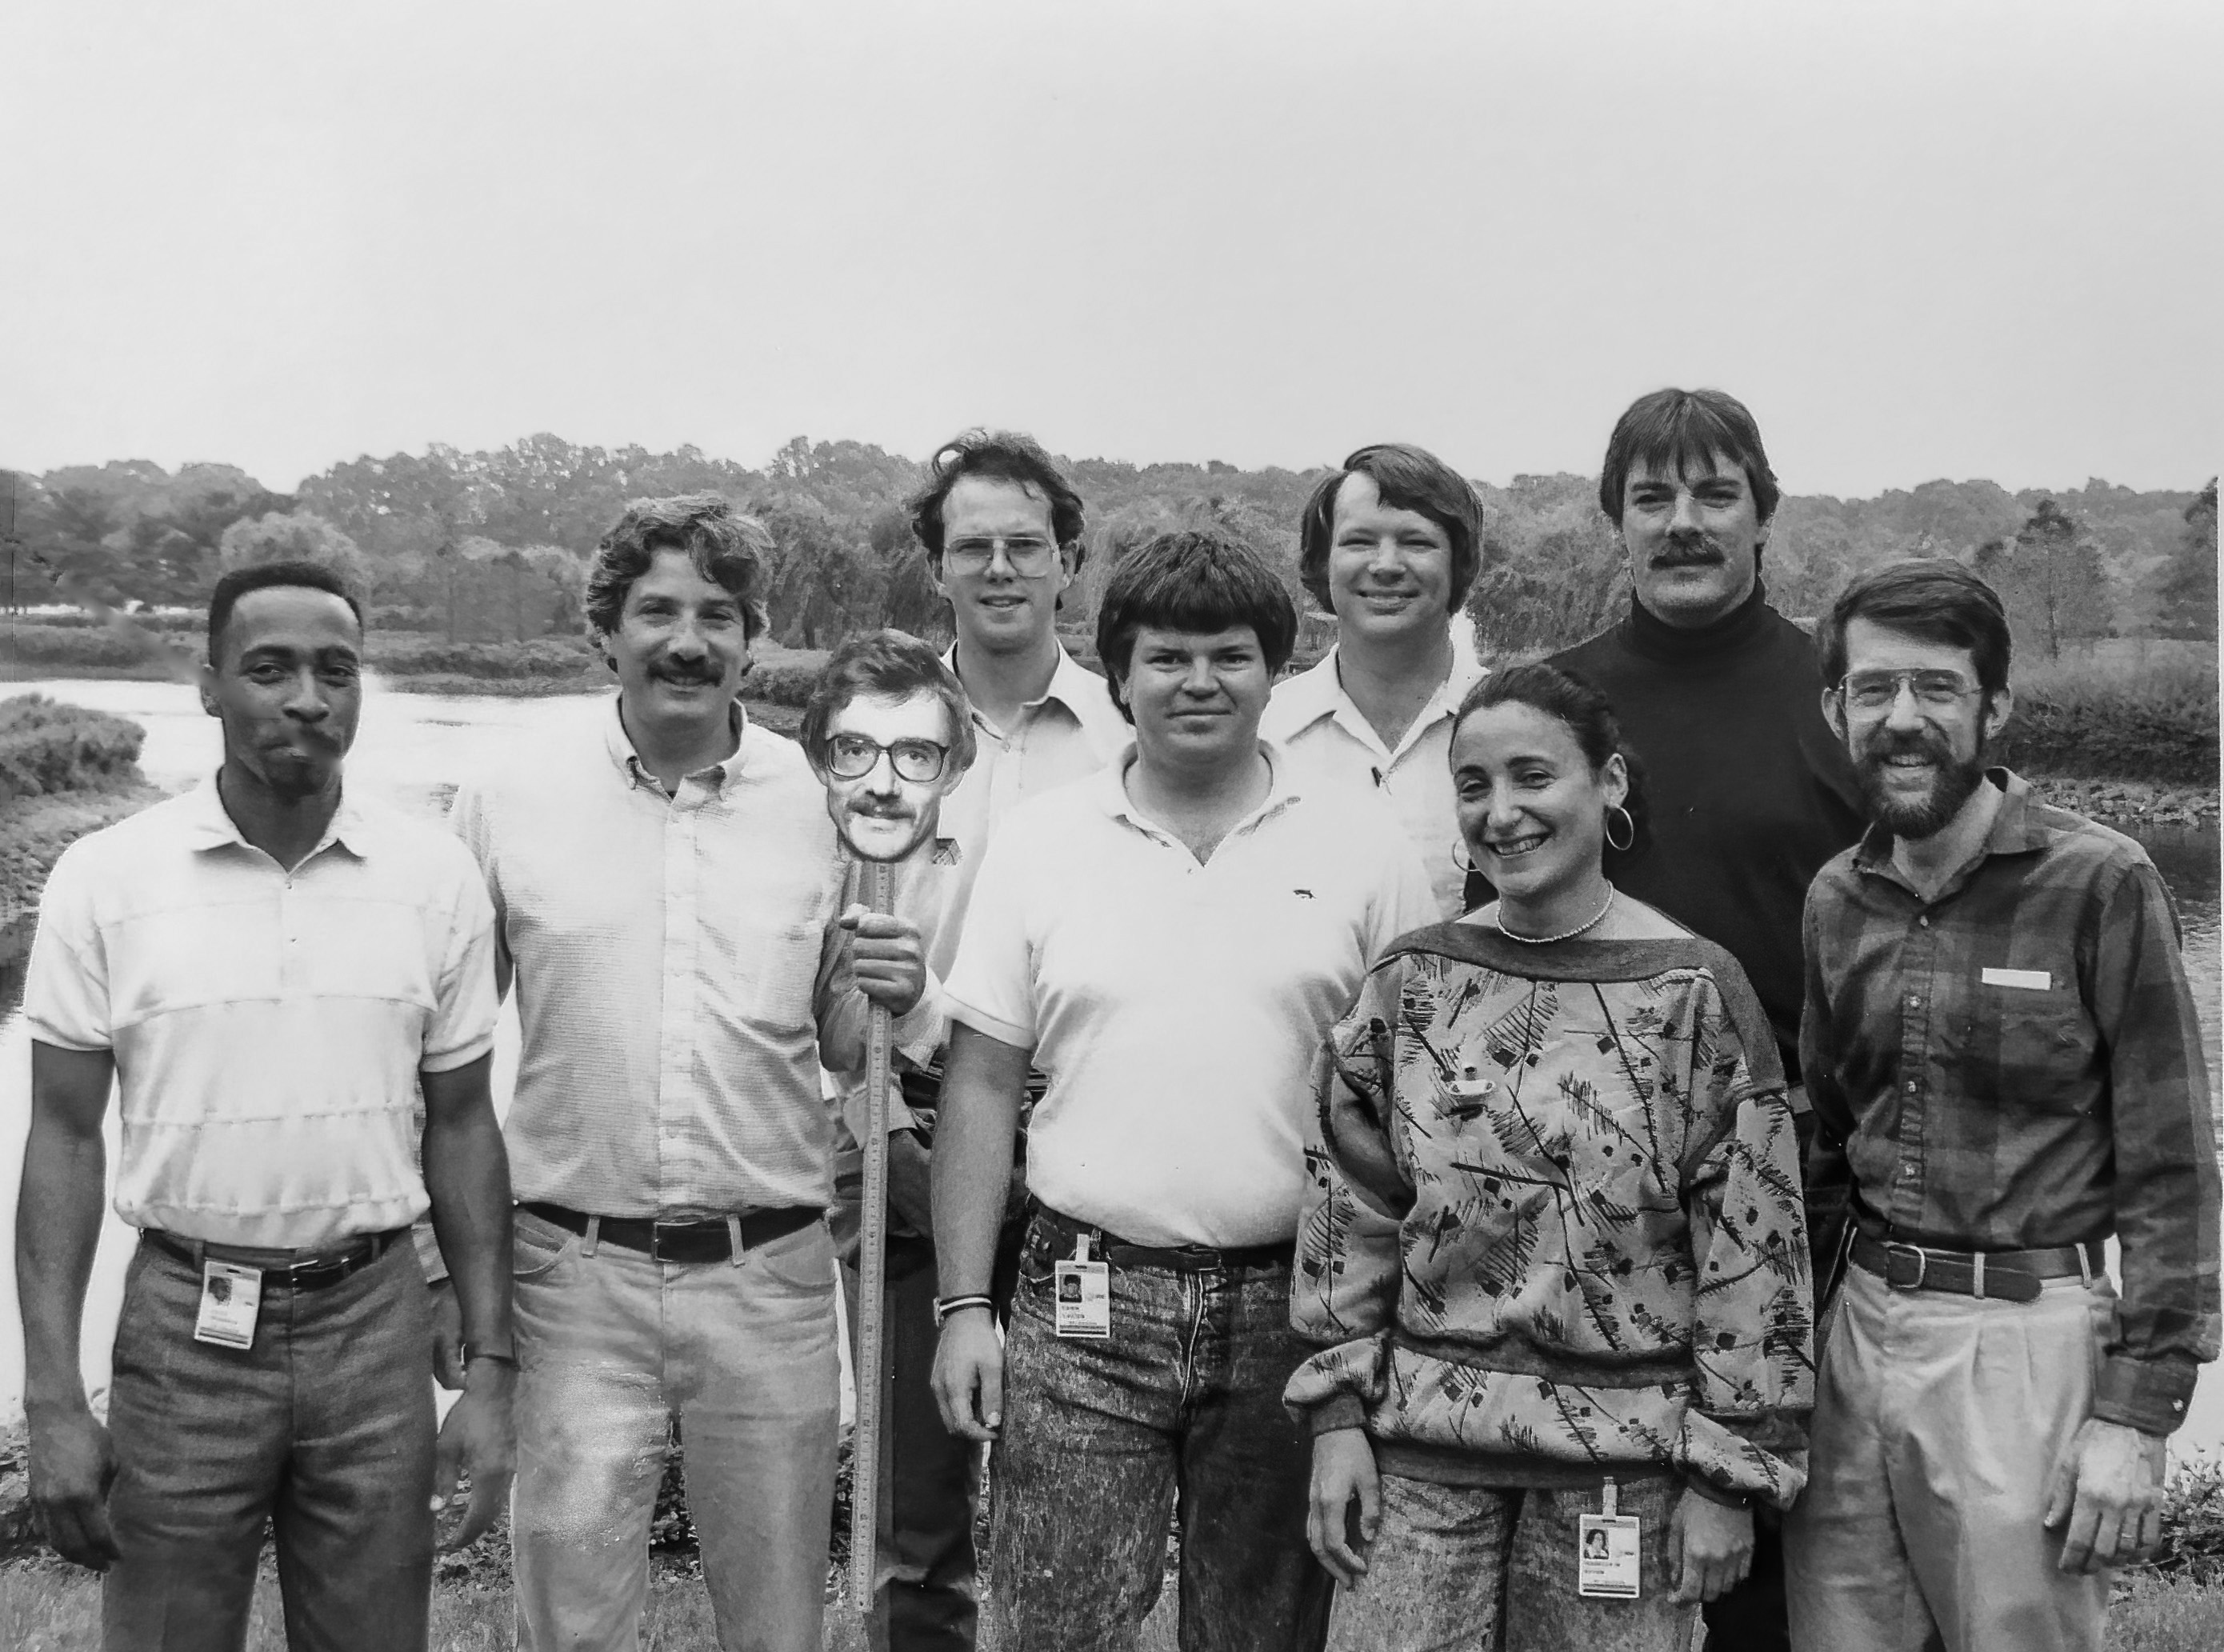
\includegraphics[width=0.65\textwidth]{figures/yann-lecun - EyIwmEDW8AIQs1C.jpeg}
    \caption{Adaptive Systems Research Department at Bell Labs 1989.\newline{}Fuente: \href{https://twitter.com/ylecun/status/1378718317695934465}{Twitter Yann Lecun}}
    \label{fig:adaptive-systems-research-department-at-bell-labs}
\end{figure}

En la década de los 90 se presentaron múltiples investigaciones y muchos avances en el campo, uno de los más importantes fue la presentación de la primera \acrshort{GAN} como una curiosidad, ya que se presentó como un duelo entre dos redes neuronales, en un principio fue un generador probabilístico y un predictor con el objetivo de maximizar la pérdida de cada uno en un juego \textit{minimax}.

En 1991 se presentó el trabajo \textit{Predictability Minimization} \cite{urgen1991learning} dichas técnicas sirvieron de inspiración para el aprendizaje por refuerzo,
En marzo de 1991 se hizo una aproximación a los \textit{transformers} con auto atención, lograron separar el conocimiento del control como una máquina clásica, pero de una forma completamente neuronal, además de gestionar actualizaciones de los pesos de forma muy rápida y eficiente.

Durante la década de 1990 las redes neuronales tendían a ser muy sencillas, con pocas capas y no muy complejas por las limitaciones técnicas de la época.
Por lo que muchos investigadores propusieron soluciones similares a las redes \acrshort{RNN} que permitían una retroalimentación, además de aceptar secuencias de información arbitraria.
Otros propusieron soluciones como la jerarquía de \acrshort{RNN} autosupervisada que aprende representaciones en distintos niveles de abstracción.
Comienzan a proponerse redes similares a las que en un futuro se llamarían \acrshort{DBN} como un método no supervisado para \acrshort{FNN}.

En junio de 1991 {Sepp Hochreiter} Figura \ref{fig:sepp-hochreiter} implemento el primer compresor de redes neuronales, además demostró uno de los principales problemas de las \acrshort{NN} el llamado problema del desvanecimiento o explosión del gradiente \ref{sec:gradient-descent} que hacía que el aprendizaje fallará.
Un análisis posterior condujo a los investigadores a una primera aproximación \acrshort{LSTM}, aunque no sería hasta 1997 con la revisión por pares y publicación del artículo \textit{Long short-term memory} \cite{hochreiter1997long} que se solucionaría parcialmente el problema.

\begin{figure}[H]
    \centering
    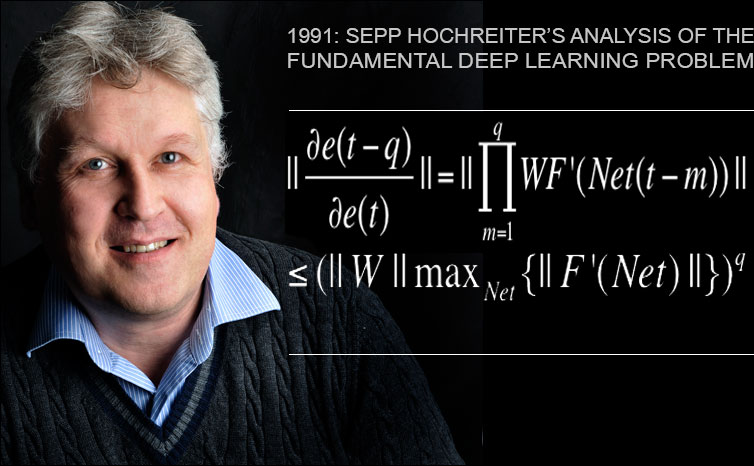
\includegraphics[width=0.65\textwidth]{figures/Sepp Hochreiter.jpg}
    \caption{Sepp Hochreiter.\newline{}Fuente: \href{https://people.idsia.ch/~juergen/fundamentaldeeplearningproblem.html}{IDSIA}}
    \label{fig:sepp-hochreiter}
\end{figure}

Más adelante, en el 2014 {Goodfellow} Figura \ref{fig:gan-ian-goodfellow} presento la primera red neuronal \gls{GAN} pura para la generación de imágenes mediante el enfrentamiento de una red neuronal generativa contra una red neuronal discriminante entrenadas con el mismo conjunto de datos \cite{goodfellow2014generative}.
Durante los próximos años se realizaron muchos aportes a las redes neuronales generativas, principalmente de paralelización de los cálculos, técnicas de estabilización, generación condiciona, arquitecturas más eficientes, funciones de pérdidas más adecuadas, aplicaciones específicas (cambiar el estilo de pintura), redes apiladas, etc.
Fruto de todo ello, {NVIDIA} en 2018 presento \gls{StyleGAN} \cite{karras2019stylebased} un modelo que es capaz de crear imágenes sintéticas de alta calidad y resolución, publicando el código en 2019 con mejoras relevantes a su primera versión.

\begin{figure}[H]
    \centering
    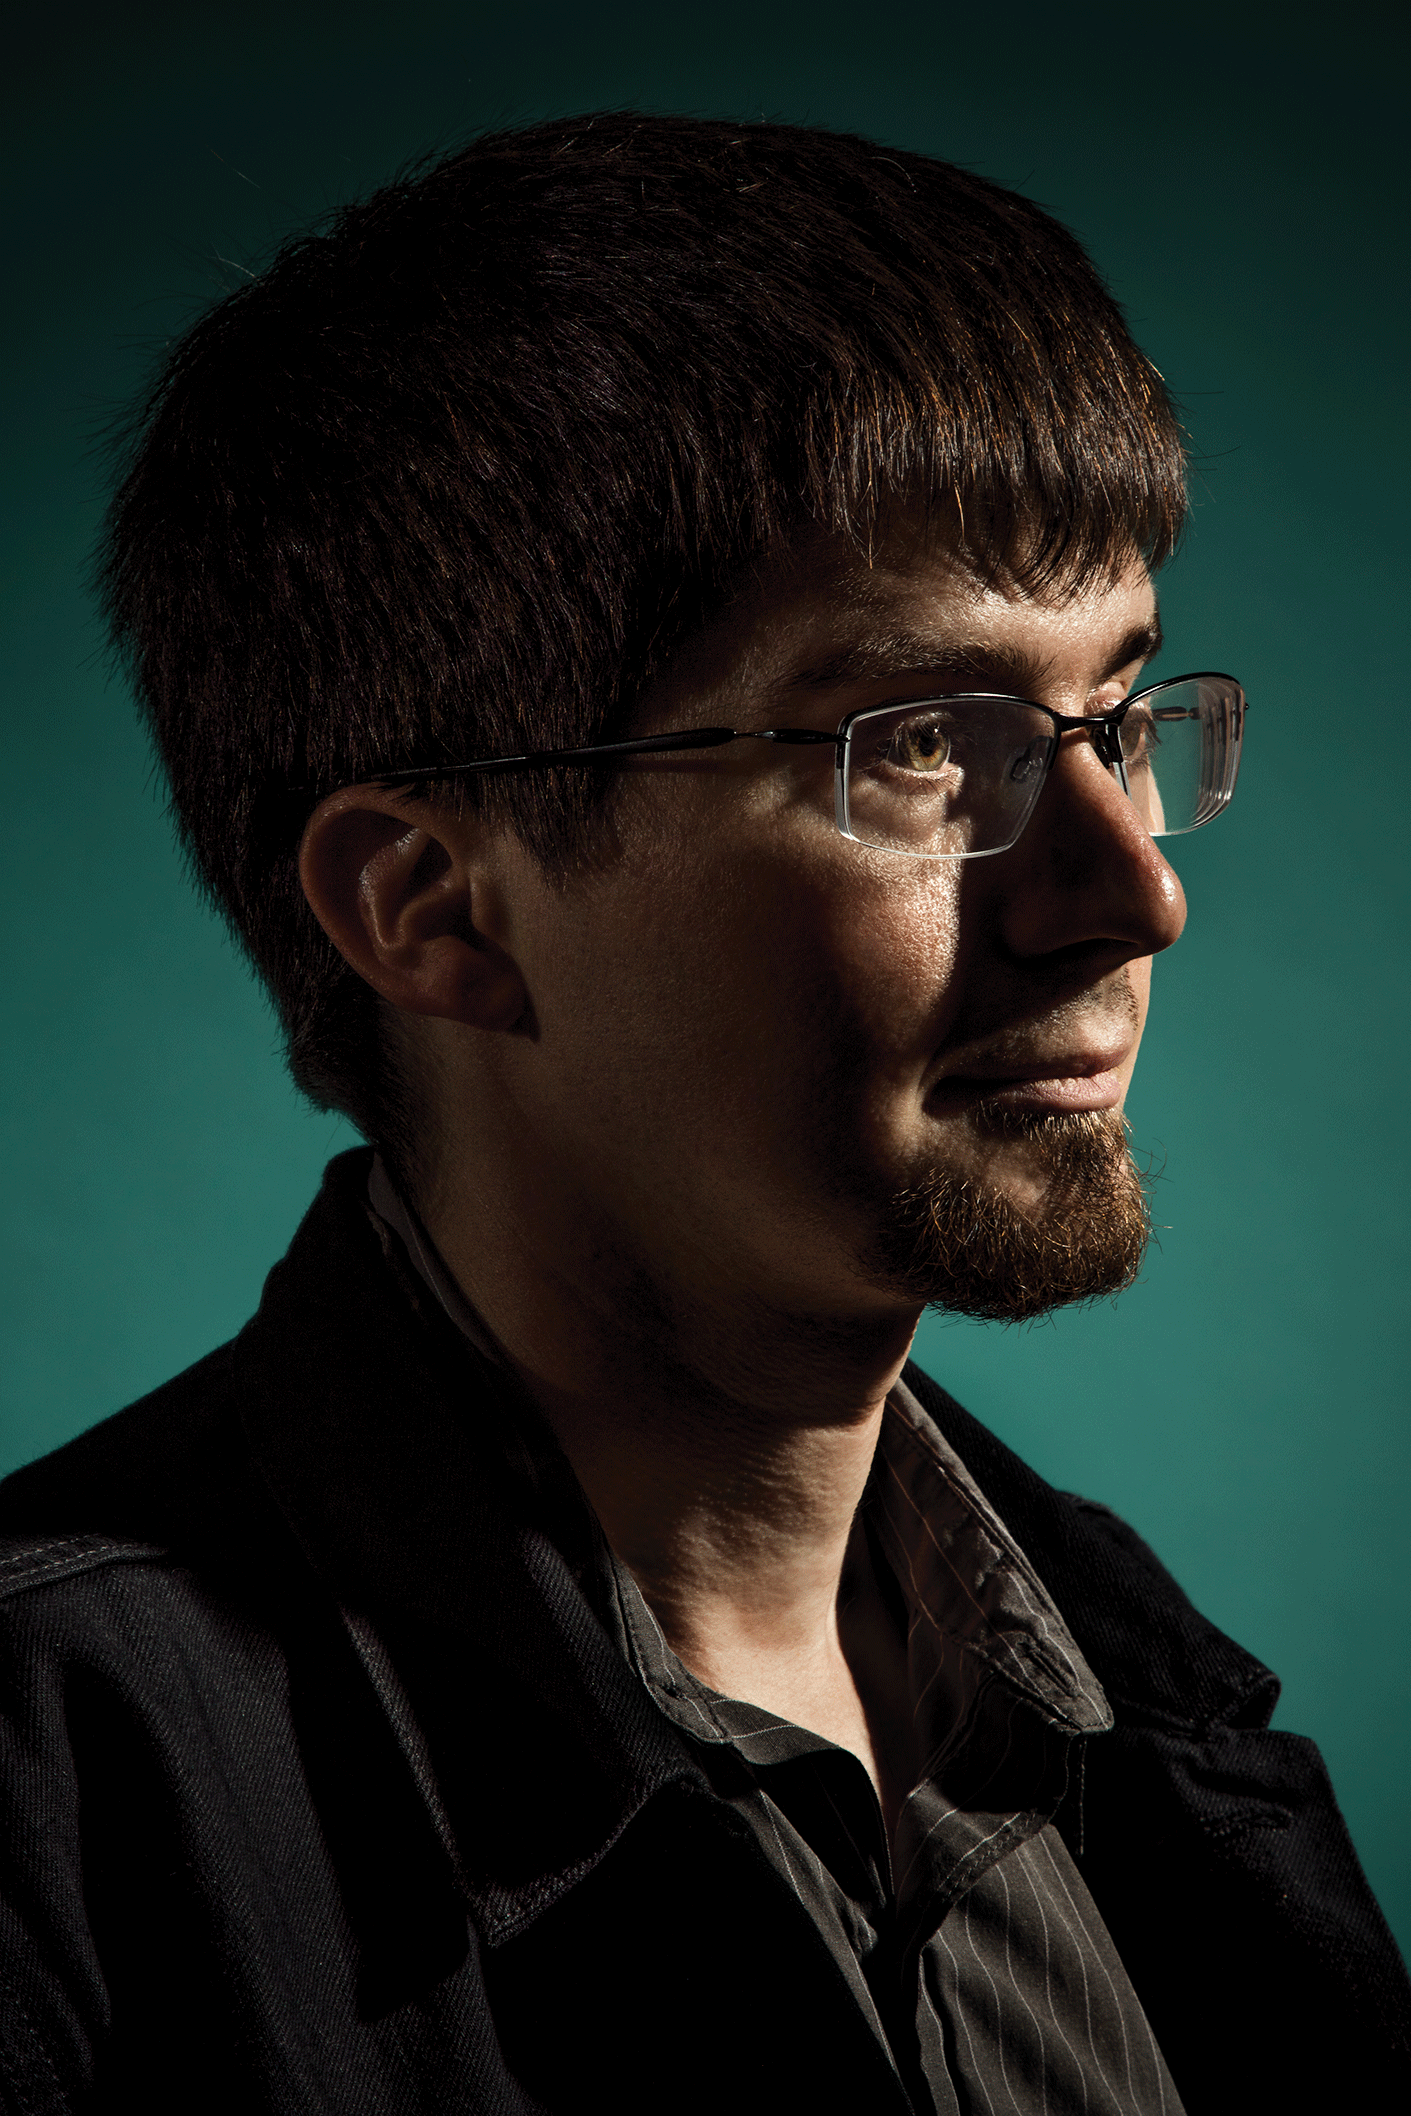
\includegraphics[width=0.2\textwidth]{figures/gan-goodfellow.png}
    \caption{Ian Goodfellow.\newline{}Fuente: \href{https://www.technologyreview.es/s/10016/el-senor-de-las-gan-el-hombre-que-dio-imaginacion-las-maquinas}{MIT Technology Review}}
    \label{fig:gan-ian-goodfellow}
\end{figure}
% endregion

